\subsection{Asking information about Public Transport Service}
The \emph{Travelndar+} System will interact with the Public Transport system, to suggest the best ride option in terms of money, time and considering the user agenda.

Several times public transport service is unavailable for many reasons, for instance an incoming strike or a maybe some metro line are stopped because of maintenance. Also in such situations the user wants to reach his appointments in time, and so the \emph{Travlendar+} System should retrieve this information from the Public Transport system, to properly schedule the user's calendar. 

\begin{table}[H]
	\centering
    
    \begin{tabular}{|p{3.5cm}|p{10.3cm}|}
    
    \hline
    \textbf{\large{Actors}}  			& \tabitem Public Transport System\\
    
    \hline
    \textbf{\large{Goals}} 				& \ref{goal:task}; \ref{goal:reachability}; \ref{goal:travel}; \ref{goal:purchase} \\
    
    \hline
    \textbf{\large{Enter Condition}}	& The \emph{Travlendar+} system starts to schedule the user's calendar\\
    
    \hline
    \textbf{\large{Events Flow}}		& \begin{enumerate}[leftmargin=0.5cm]
                                          	\item The \emph{Travlendar+} System asks mobility information or travel cards information to the \emph{Public Transport} system through existing APIs
                                          	\item The \emph{Public Transport} system sends back all the required information that the \emph{Travlendar+} service has requested
                                          \end{enumerate}
    										\\
    \hline
    \textbf{\large{Exit Condition}} 	& The \emph{Travlendar+} system has requested all the mobility information it needed from the \emph{Public Transport} service\\
    
    \hline
    \textbf{\large{Exception}} 			& It can be happened that either the \emph{Public Transport} service is unavailable or an information request is rejected. In the former case it is impossible knowing useful information in order to schedule the user's calendar, so the \emph{Travlendar+} system will compute a calendar without those information; otherwise in the latter case our system tries to ask again the information it needs\\
    
    \hline
    
    
    \end{tabular}
	
\end{table}

\begin{figure}[H]
\centering
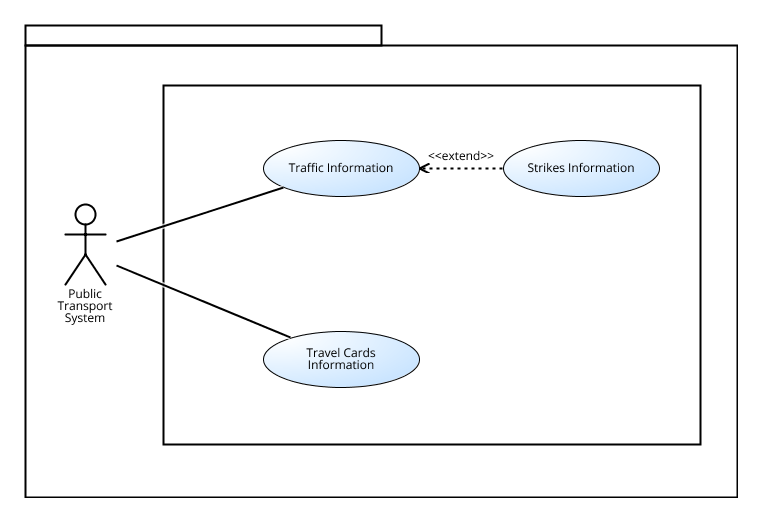
\includegraphics[scale=0.5]{Pictures/UseCaseDiagram/ATM.png}
\caption{UML Use Case Diagram for the information requests asked to the \emph{Public Transport} service}
\end{figure}